\subsection{A stochastic model of human-machine interaction for learning dialog strategies \cite{Levin2000A}}

This paper proposes a quantitative model for dialog systems that can be used for learning the dialog strategy. After formalising the dialog design as a \emph{Markov decision process (MDP)}, the reinforcement learning algorithm is used to find the optimal strategy. This approach is evaluated in an \emph{air travel information system (ATIS)} task.

The key idea of this paper is to formalise the dialog design as an optimization problem with an objective function reflecting different dialog dimensions for a given application. With some assumptions about the state transition probabilities and cost assignment, a dialog system can be mapped to a MDP, which has a variety of data driven algorithms for finding the optimal strategy.

The first step is to state the problem of dialog design as optimization of an objective $C$:
$$C = \sum W_i \langle C_i \rangle,$$
where the terms $\langle C_i \rangle$ are the expected costs for different dialog dimensions. The paper illustrates the concepts with a toy example of ``Day-and-Month Dialog'', where the goal is to get the correct day and month values from the user. In the case, the objective $C$ has three components: the first part denotes the \emph{expected duration} of the dialog; the second part denotes the expected number of error; the last part corresponds to the expected distance from achieving the application goal. With this concept, the goal of a dialog system is to minimize the cost function.

\begin{figure}[htbp]
  \centering
  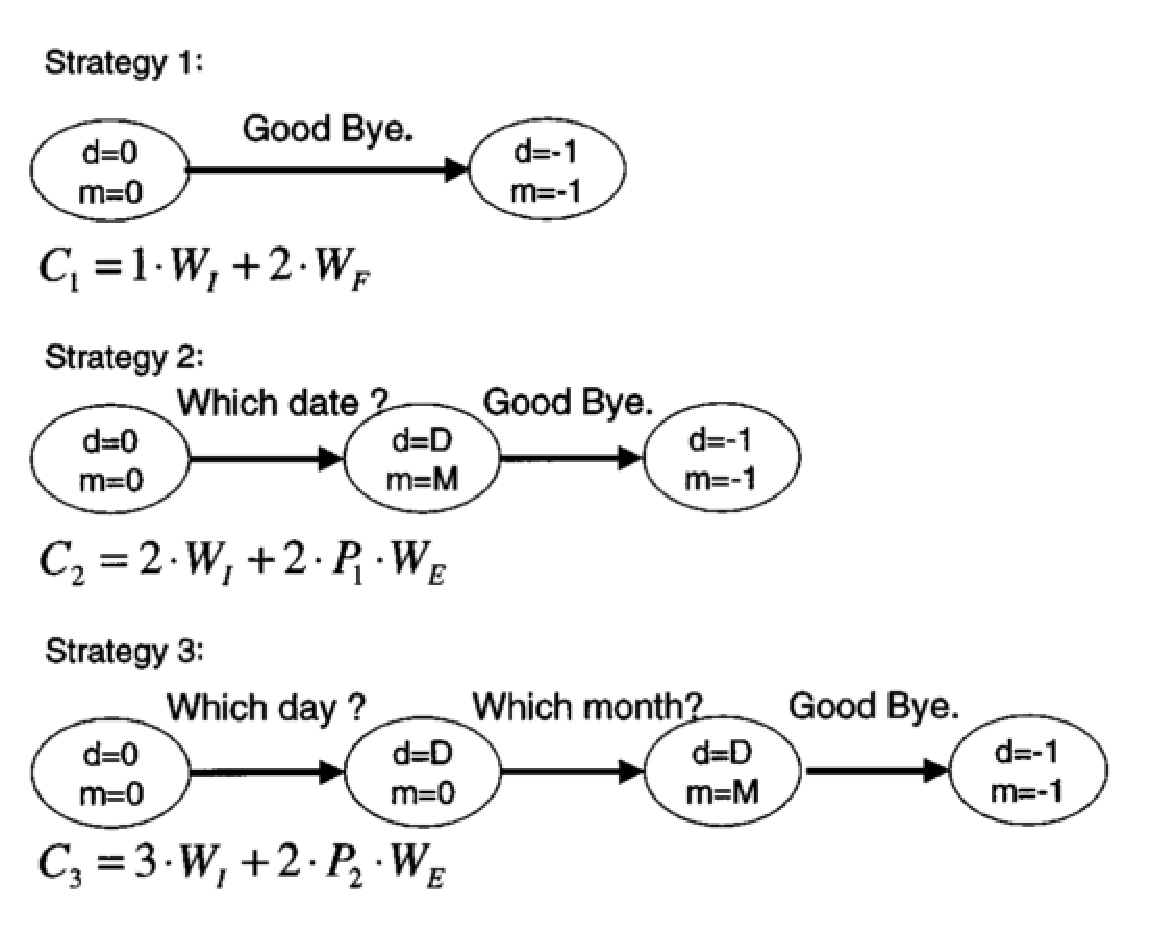
\includegraphics[width=.6\linewidth]{10_17_dialog_MDP1}\\
  \caption{Three possible strategies for the day-month dialog system}\label{fig:dialog_MDP1}
\end{figure}

The next step is to formalize a dialog system as a sequential decision process in terms of its action set, state space, and strategies: 1) The action set of the dialog system includes all possible actions it can perform, such as interactions with the user (e.g., asking the user for input, providing some output, etc.). In the toy example, there are four actions, such as asking for the day $A_d$, asking the month $A_m$, asking the date (day and month) $A_{dm}$, and a final action $A_f$; 2) The state $s$ includes the values of all relevant variables that determine the next action. In the example each state has two integer variables, $d \in \{0, ..., 31\}$ and $m \in \{0, ..., 12\}$, corresponding to the day and month respectively. 3) A dialog strategy maps each state to an action. For example, Figure \ref{fig:dialog_MDP1} shows three possible strategies for the example system.

With some assumptions about the transition probabilities between states, and the cost assignment, the sequential decision process can be formalise as a MDP. Then the optimal strategy can be obtained by a variety of reinforcement learning algorithms.

However, in reinforcement learning, the optimal strategy is learned not from a static corpus but through interaction, because the strategy itself determines the distribution of states in the corpus. To overcome this problem, the paper proposes the use of a \emph{simulated user}. The simulated user is a stochastic generative model that produces speech acts as a response to a dialog action. The simulated user does not deal with the language understanding component - it communicates with the dialog system through semantic representations. The parameters of the simulated user can be estimated from an annotated dialog corpus.

\begin{figure}[htbp]
  \centering
  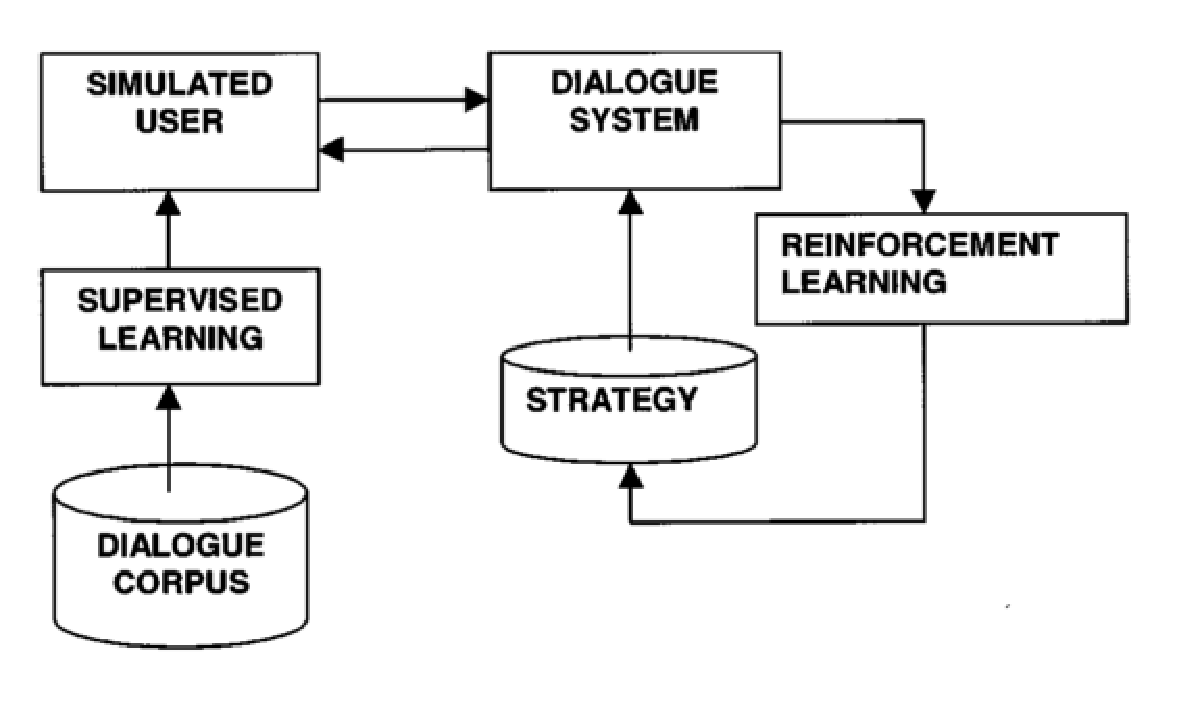
\includegraphics[width=.6\linewidth]{10_17_dialog_MDP2}\\
  \caption{Procedural description of the learning paradigm}\label{fig:dialog_MDP2}
\end{figure}

Once a simulated user is available, it can be used in a generative mode for interacting with the dialog system while the reinforcement learning algorithm is estimating the optimal strategy. Then when a reasonable estimate of the optimal strategy is obtained, the system can be used with real users and the learning process can continue. Figure \ref{fig:dialog_MDP2} summarizes the suggested learning paradigm.

\begin{figure}[htbp]
  \centering
  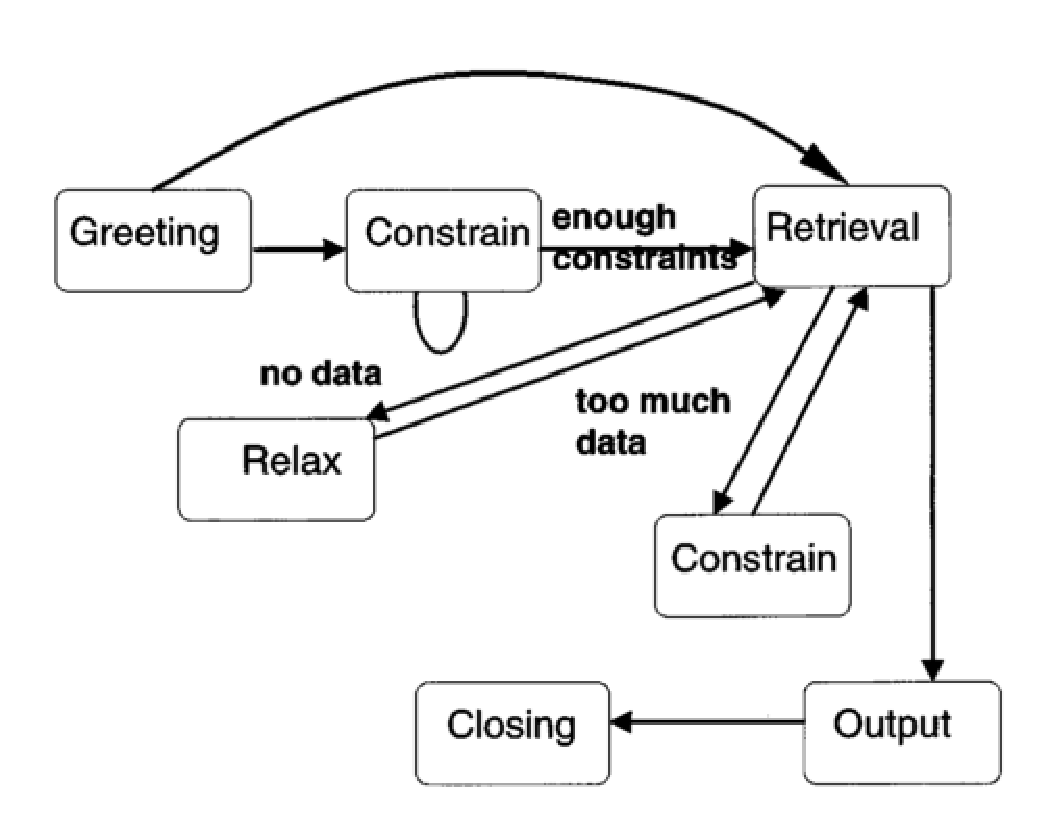
\includegraphics[width=.5\linewidth]{10_17_dialog_MDP3}\\
  \caption{Schematic representation of the optimal strategy for ATIS}\label{fig:dialog_MDP3}
\end{figure}

In the experimental study, the paper shows that a nontrivial strategy can be automatically learned given the simple objective function. For example, Figure \ref{fig:dialog_MDP3} shows the learned strategy of the ATIS task.

Remark: I have also considered formalising the dialog manager as a MDP, and realised one obvious difficulty is that there is not an interactive environment to train the system. This paper introduces simulated users to overcome this difficulty. Another good idea is to abstract the dialog process, such as using semantic representations without considering the ASR or NLU component. I think this paper shows a very promising approach for building our chatbot. 